\chapter{Umsetzung}
\label{ch:S5_Umsetzung}

\section{Erläuterung des Softwaretechnischen Entwurfs}

Für die Softwaretechnische Umsetzung wurden zunächst die Anforderungen an das Geogameframework in Kapitel \ref{ch4:s:Lösungen} sowie die gewählte Lösung aus Kapitel \ref{ch4:s:choosen_solution} im Detail evaluiert. Für die Umsetzung des Entwurfs wurde zunächst ein Entwurfs des Prozesses identifiziert, welcher die Geodaten aus OSM bis hin zur Darstellung im Beispielspiel darstellt. Eine Visualisierung ist in Abbildung \ref{img:ch5_img01_framework_progress} zu sehen.
\\\\

\begin{figure}[H]
\begin{center}
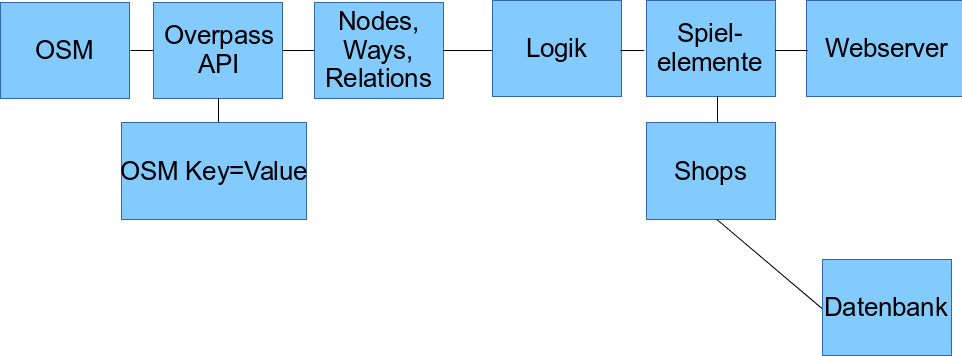
\includegraphics[width=140mm]{images/ch5_img01_framework_progress.png}
\caption{Prozess: Von OSM zum Spielelement}
\label{img:ch5_img01_framework_progress}
\end{center}
\end{figure}

Zunächst steht zu Beginn des Prozess als Datengrundlage Openstreetmaps.
Die Daten werden allerdings nicht direkt von OSM über die OSM API abgerufen, sondern über Overpass. Das liegt daran, dass die OSM API selbst nur sehr rudimentäre Abfragen erlaubt.
Stattdessen wird die Overpass API verwendet, da sie geografische Abfragen erlaubt \cite{Meyer.2013}. 


\section{Bewertung der Technologien und Werkzeuge}

\section{Implementierung des Geogameframeworks}